\documentclass{article}
\usepackage{graphicx} % Required for inserting images
\usepackage{amsmath, amssymb, amsthm}
\title{
    \vspace{-2cm} % adjust spacing if needed
    
\includegraphics[width=0.1\textwidth]{images/logo.png} \\[0.5cm] % logo above title
    Celestial Mechanics II
}
\author{Sheikh Hasin Abrar}
\date{January 11, 2026}
\usepackage[a4paper, left=2cm, right=2cm, top=2.5cm, bottom=2.5cm]{geometry}
\usepackage{tcolorbox}
\tcbuselibrary{breakable}
\usepackage{caption}
\usepackage{graphicx}
\captionsetup[figure]{labelformat=empty}
\begin{document}
\maketitle
\section{Introduction}
In the previous sections of Celestial Mechanics, we discussed Newton’s law of gravitation, angular momentum, and the conservation of mechanical energy for different orbital configurations. We also applied these concepts through problem-solving.
In this section, we extend those ideas by introducing the empirical relations that describe planetary motion. The three laws, known as Kepler’s Laws, provide the geometric and kinematic framework that governs how celestial bodies move in their orbits.
\section{Kepler's Laws}
Based on the precise observations made by the Danish astronomer Tycho Brahe, Johannes Kepler spent sixteen years determining the parameters of planetary orbits, starting with Mars and later extending his analysis to the Earth. The transition from raw observational data to empirical laws was far from straightforward, as each planet’s motion had to be understood relative to the Earth, which itself revolves around the Sun. Through meticulous analysis and countless revisions, Kepler eventually identified consistent mathematical relationships governing planetary motion.  \hfill [Fundamental of Astronomy]
\\[1EM]
These laws remain fundamental to modern astrophysics, as they enable the prediction of orbital motion, the estimation of distances and periods, and the understanding of how gravitational forces govern the dynamics of celestial bodies. 
\\[1EM]
Kepler’s analysis of the planetary motion can be summarized in
three laws:
\begin{enumerate}
    \item All planets move in elliptical orbits, with the Sun at one focus.
    \item The radius vector joining any planet to the Sun sweeps out equal areas in equal times.
    \item The square of the orbital period of any planet is directly proportional to the cube of the semi-major axis of its orbit.
\end{enumerate}


\subsection{First Law}
Kepler’s first law of planetary motion states that the orbit of a planet is an ellipse with the Sun at one of its foci. This is a specific case of a more general principle: all objects in closed orbits around a central body follow elliptical paths with the central body at one focus. Also open orbits such as hyperbolas or parabolas also have the central body located at a focus, but the objects do not return, instead escaping the system.
\\
\begin{center}
    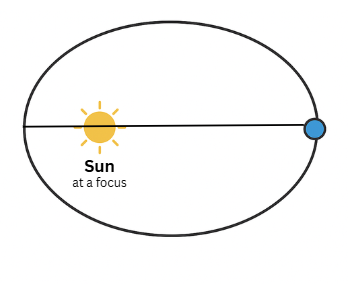
\includegraphics[width=0.3\textwidth]{images/First.png}
\end{center}
\newpage
\begin{tcolorbox}[breakable,colback=red!5!white, colframe=red!75!black, title={Derivation of 1st Law}]|
Now, let us examine the proof of the \textbf{First Law}, which involves a brief calculus-based derivation.  

We begin with Newton’s Second Law, \( \vec{F} = m\vec{a} \).  
For a planet of mass \( m \) orbiting a much larger mass \( M \), the gravitational force acts radially inward and is given by  

\[
\vec{F} = -\frac{GMm}{r^2}\hat{r}
\]

The acceleration has both radial and transverse (angular) components. Even if the planet moves in a circular orbit where \( r \) remains constant, it still experiences an inward acceleration of \( r\omega^2 \) (equivalently \( v^2 / r \)).  

Therefore, the total radial acceleration can be expressed as  

\[
\frac{d^2r}{dt^2} - r\omega^2 = -\frac{GM}{r^2}
\]
This equation represents the balance between the gravitational attraction and the combined effects of radial and angular acceleration in orbital motion. 
\\
But we can't integrate this yet, because $\omega$ varies as well. However, since the angular momentum $L$ is constant, 
\[
L = m r^2 \omega,
\]
we can eliminate $\omega$ from the equation to obtain:
\[
\frac{d^2 r}{dt^2} = -\frac{GM}{r^2} + r \left( \frac{L}{m r^2} \right)^2
\]
\[
= -\frac{GM}{r^2} + \frac{L^2}{m^2 r^3}
\]
Now, if we consider $\mu$ as the \textbf{reduced mass}, the equation becomes:

\[
\frac{d^2 r}{dt^2} = -\frac{GM}{r^2} + \frac{L^2}{\mu^2 r^3}
\] 
\\ 
This equation can be integrated using two clever substitutions.
The first involves replacing the variable $r$ with its inverse, $u = \frac{1}{r}$. 
The second uses the constancy of angular momentum to transform the independent variable from time $t$ to the angular coordinate $\theta$. 
\[
L = \mu r^2 \omega = \mu r^2 \frac{d\theta}{dt} = \frac{\mu}{u^2} \frac{d\theta}{dt}
\]
so
\[
\frac{d}{dt} = \frac{L u^2}{\mu} \frac{d}{d\theta}.
\]

Therefore,

\[
\frac{dr}{dt} = \frac{d}{dt}\left(\frac{1}{u}\right) = -\frac{1}{u^2} \frac{du}{dt} 
= -\frac{L}{\mu} \frac{du}{d\theta},
\]
\[
\frac{d^2 r}{dt^2} = -\frac{L^2 u^2}{\mu^2} \frac{d^2 u}{d\theta^2}.
\]
Substituting in the equation of motion gives:
$$
\frac{d^2u}{d\theta^2} + u = \frac{GM\mu^2}{L^2}
$$
Solving the equation we get
$$
u = \frac{1}{r} = \frac{GM\mu^2}{L^2} + A\cos\theta
$$
where $A$ is a constant of integration, determined by the initial conditions. 
\newpage
Combining most of the constants using suitable substitutions, we can simplify the equation as follows:
$$
\frac{a(1-e^2)}{r} = 1 + e\cos\theta
$$
This is equivalent to the standard $(r, \theta)$ equation of an ellipse of semi major axis $a$ and eccentricity $e$, with the origin at one focus. 
Hence we have proven Kepler's First Law. 
\end{tcolorbox}
\subsection{Second Law}
 Kepler's Second Law states that a line segment joining a planet and the sun sweeps out equal areas during equal intervals of time. This implies that the planet moves faster when it is closer to the Sun and slower when it is farther away.
 \\[2EM]
 \begin{center}
    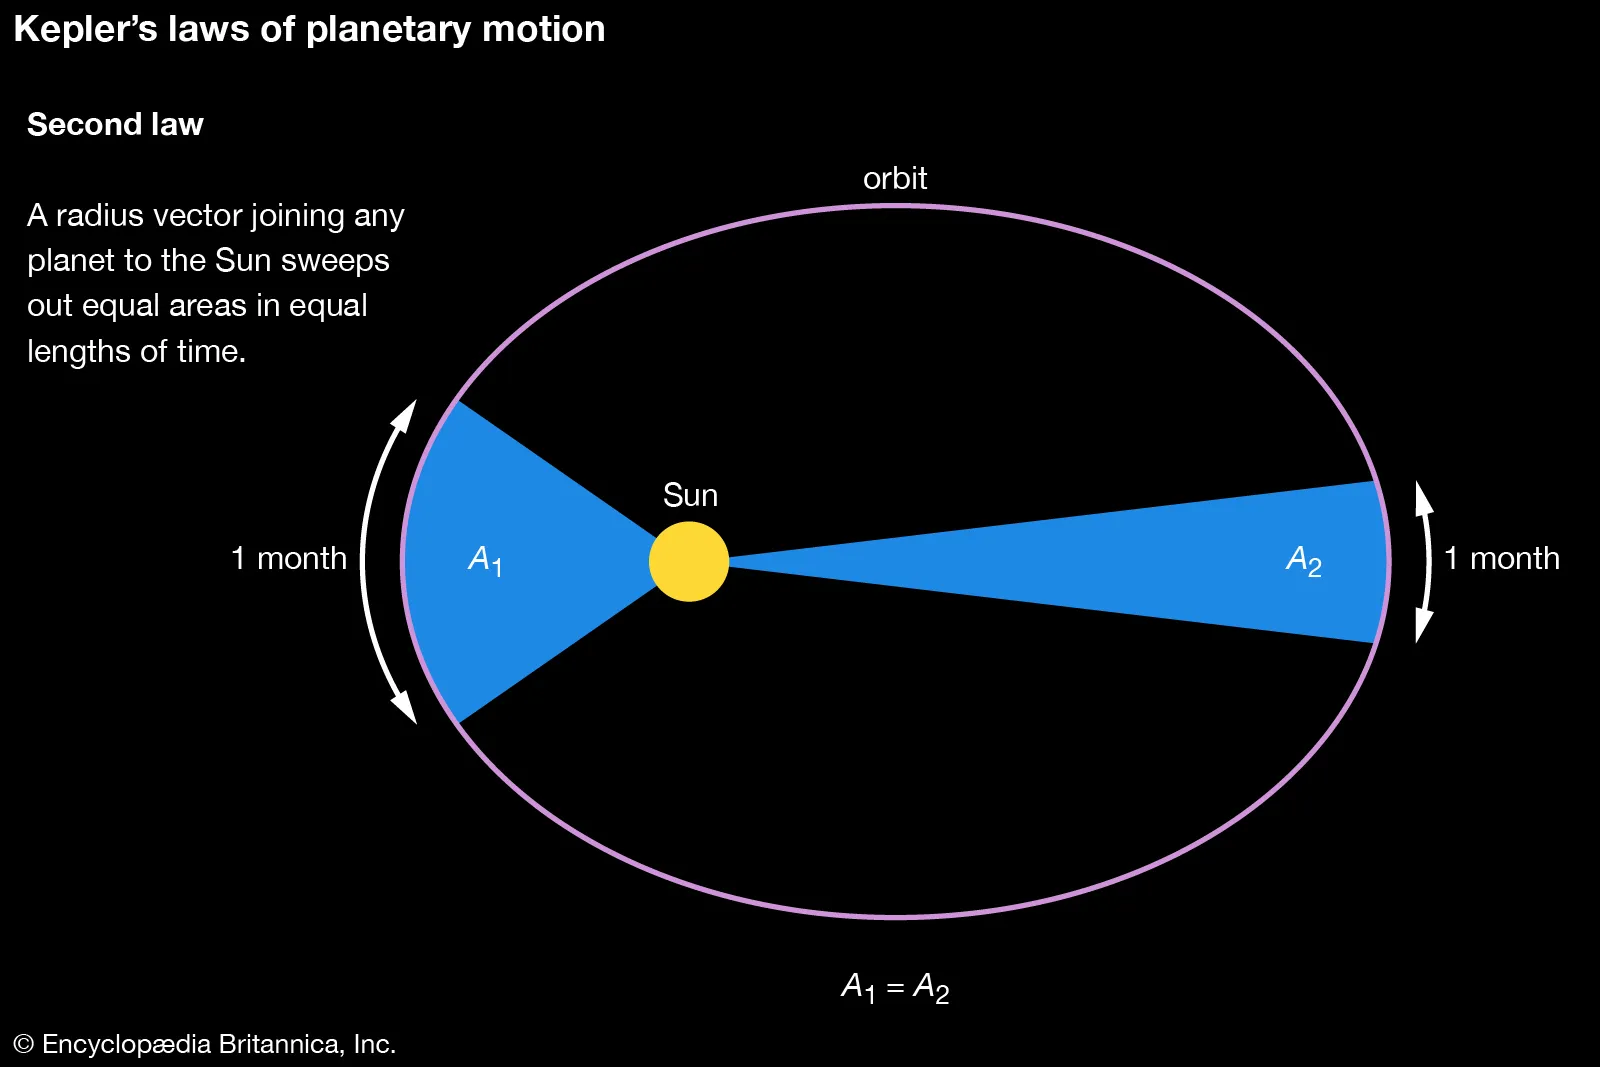
\includegraphics[width=0.8\textwidth]{images/Keplers 2nd Law.png}
\end{center}
\vspace{3em}
Before diving into the mathematical framework of Kepler's Second Law, we must review a few essential related concepts.
\\[1EM]
\textbf{Angular Momentum:}  
From the previous handout, you already know that the angular momentum of a particle is defined as the vector product of its position vector and its linear momentum. In symbols,
\[
\vec{L} = \vec{r} \times m\vec{v}.
\]
It measures the rotational motion of a body with respect to a chosen origin.
\\ [1em]
\textbf{Torque:}  
Torque is defined, with respect to a fixed origin, as the vector product of the position vector and the force acting on the body:
\[
\vec{\tau} = \vec{r} \times \vec{F}.
\]
It represents the tendency of a force to produce rotational motion.
\\
Connecting them, we have
\[
\frac{d\vec{L}}{dt} = \vec{\tau}.
\]
\begin{tcolorbox}[breakable,colback=red!5!white, colframe=red!75!black, title={Derivation of 2nd Law}]|
\begin{center}
    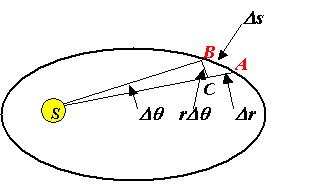
\includegraphics[width=0.5\textwidth]{images/2nd law.jpg}
\end{center}
According to the figure, after an infinitesimal time \(dt\), the planet moves a small distance
\[
ds = v\,dt
\]
along its orbit. Since \( \delta s\) is very small compared to \(r\),
the angle \(\theta\) between the radius vector and the velocity vector is also
very small.

The area swept out by the radius vector joining the planet to the Sun during
this interval is equal to the area of triangle \(ABS\)
Thus, the infinitesimal area swept out in time \(dt\) is
\[
dA = \frac{1}{2} ds \, r \sin\theta
    = \frac{1}{2} r v \sin\theta \, dt.
\]
As we have learnt from definition of angular momentum,
\[
L = m r v \sin\theta,
\]
it follows that
\[
r v \sin\theta = \frac{L}{m}.
\] 

Substituting this into the expression for \(dA\) gives
Rewriting the expression, we obtain
\[
\frac{dA}{dt} = \frac{L}{2m}.
\] \hfill [1]
As we saw before, torque is defined as
\[
\vec{\tau} = \vec{r} \times \vec{F}.
\]
Since the only force acting on the planet is gravity, \(\vec{F}\) is always 
\emph{parallel} to \(\vec{r}\) (both point along the radial direction). 
Therefore, the cross product becomes
\[
\tau = rF \sin\theta,
\]
and because the angle between \(\vec{r}\) and \(\vec{F}\) is \(\theta = 0\),
\[
\tau = 0.
\]

Hence,
\[
\frac{d\vec{L}}{dt} = 0,
\]
which shows that the angular momentum \(\vec{L}\) remains constant.

Going back to [1], since since we have shown L is constant and mass m is also constant so $\frac{dA}{dt}$ is also constant, thus proving Kepler's second Law. 
\end{tcolorbox}
\newpage
\noindent
We can relate the time $t$ that a planet takes to cover an area $A_s$ through a simple proportionality. 
The ratio of the area swept to the total area equals the ratio of the time elapsed to the total period:
\[
\frac{t}{T} = \frac{A_s}{A},
\]
where $T$ is the period of revolution and $A = \pi a b$ is the total area of the elliptical orbit.
\\
\begin{tcolorbox}[breakable,colback=green!5!white, colframe=green!75!black, title={Problem}]

A Sun--orbiting periodic comet is the farthest from the Sun at $31.5\,\text{AU}$
and the closest at $0.5\,\text{AU}$. If the orbital period of this comet is 
$64$ years, what is the area (in $\text{AU}^2/\text{year}$) swept by the line 
joining the comet and the Sun?\hfill [(I07 - T07 - A)]
\end{tcolorbox}
\begin{tcolorbox}[breakable,colback=green!5!white, colframe=green!75!black, title={Solution}]
\noindent
This comet has a period of 64 years and a semi--major axis measuring 16 AU.

\medskip

\noindent
By Kepler's second law, the comet will sweep equal areas in equal times.

\[
\text{Area per year}
  = \frac{\text{Area of elliptical orbit}}{T}
  = \frac{\pi a b}{T}
\]

\bigskip
\noindent
The perihelion distance is given by
\[
a(1-e) = 0.5\ \text{AU},
\]
where \(e\) is the eccentricity.

\[
b^2 = a^2(1-e^2) = a^2 - a^2 e^2
\]
\[
= (a+ae)(a-ae)
\]
\[
= (\text{aphelion distance}) \times (\text{perihelion distance})
\]

\[
b^2 = 31.5 \times 0.5
\]
\[
\Rightarrow\ b = 3.97\ \text{AU}
\]

\[
\therefore\ 
\text{Area per year}
= \frac{\pi \times 16 \times 3.97}{64}
= 3.1\ (\text{AU})^2/\text{yr}.
\]
\end{tcolorbox}
\newpage
\noindent
\textbf{Elliptical Orbit Parameters:}
This part is purely based on conic sections which you have learnt in your highschool. But if you haven't already then don't worry we got you this. \\
\begin{figure}[h!]
    \centering
    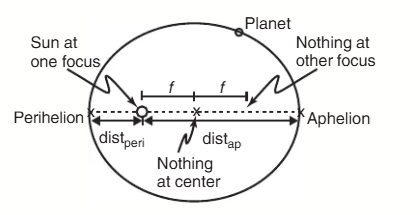
\includegraphics[width=0.5\textwidth]{images/Orbital.png}
    \caption*{\small Source: \textit{A Student's Guide to the Mathematics of Astronomy}}
\end{figure}
\\[1EM]
The point in a planet’s orbit that is closest to the Sun is called the \textit{perihelion}, 
and the point farthest from the Sun is called the \textit{aphelion}. From the geometry of 
an elliptical orbit, the sum of these two distances is constant. If the distance from the 
Sun at perihelion is $\text{dist}_{\text{peri}}$ and the distance at aphelion is 
$\text{dist}_{\text{ap}}$, then

\begin{equation*}
    \text{dist}_{\text{peri}} + \text{dist}_{\text{ap}} = 2a.
\end{equation*}
\\ 
Here a is the semi-major axis of the elliptical orbit. 
\\
Considering the geometry of an ellipse, the Sun lies at one of the two foci,
a distance $f$ from the center. Therefore, the distances from the Sun to the 
planet at aphelion and perihelion are

\[
\text{dist}_{\text{ap}} = a + f, \qquad
\text{dist}_{\text{peri}} = a - f.
\]
\\
Since the eccentricity is defined as $e = \frac{f}{a}$, it follows that $f = ae$.
Substituting this into the expressions above gives
\[
\text{dist}_{\text{ap}} = a(1 + e), \qquad
\text{dist}_{\text{peri}} = a(1 - e).
\]
\\
If we add the expressions for the aphelion and perihelion distances, we obtain
\[
\text{dist}_{\text{ap}} + \text{dist}_{\text{peri}} = 2a.
\]
\\
Thus, the sum of the distances from the Sun at aphelion and perihelion is twice
the semi-major axis which we saw before. 
\\
Similarly, subtracting the two expressions gives
\[
\text{dist}_{\text{ap}} - \text{dist}_{\text{peri}} = 2ae = 2f
\]
\\\
which means twice the focal distance of the ellipse.
We can also express the eccentricity in terms of the aphelion and perihelion
distances. Using the relations above, we obtain

\[
e = \frac{a(1+e) - a(1-e)}{a(1+e) + a(1-e)}
  = \frac{\text{dist}_{\text{ap}} - \text{dist}_{\text{peri}}}
         {\text{dist}_{\text{ap}} + \text{dist}_{\text{peri}}}.
\]
\newpage
\noindent
Below you can find all the relations of all orbital relations found in elliptical oprbits. 
\\[1EM]
\begin{table}[h]
\centering
\begin{tabular}{lll}
\hline
\textbf{To find} & \textbf{If you know} & \textbf{Use} \\
\hline
$dist_{ap}$ & $a$ and $e$ & $dist_{ap} = a(1+e)$ \\
\\[1EM]
$dist_{peri}$ & $a$ and $e$ & $dist_{peri} = a(1-e)$ \\
\\[1EM]
$a$ & $dist_{ap}$ and $dist_{peri}$ & $2a = dist_{ap} + dist_{peri}$ \\
\\[1EM]
$e$ & $dist_{ap}$ and $dist_{peri}$ &
$e = \dfrac{dist_{ap} - dist_{peri}}{dist_{ap} + dist_{peri}}$ \\
\\[1EM]
$f$ & $a$ and $e$ & $f = ae$ \\
\\[1EM]
$f$ & $a$ and $b$ & $f = \sqrt{a^2 - b^2}$ \\
\\[1EM]
$f$ & $dist_{ap}$ and $dist_{peri}$ & $2f = dist_{ap} - dist_{peri}$ \\
\\[1EM]
$e$ & $a$ and $b$ & $e = \sqrt{1 - \dfrac{b^2}{a^2}}$ \\
\\[1EM]
$e$ & $a$ and $f$ & $e = \dfrac{f}{a}$ \\
\\[1EM]
$b$ & $e$ and $a$ & $b = a\sqrt{1-e^2}$ \\
\\[1EM]
$a$ & $e$ and $b$ & $a = \dfrac{b}{\sqrt{1-e^2}}$ \\
\hline
\end{tabular}
\end{table}
\newpage
\subsection{Third Law}
Kepler’s third law of planetary motion states that for elleptical orbits the square of the period of revolution of a planet is directly proportional to the cube of the semi-major axis of its orbit.
So planets far from the Sun take longer to complete one orbit than planets close to the Sun.
$$T^2 \propto a^3 $$
\begin{tcolorbox}[breakable,colback=red!5!white, colframe=red!75!black, title={Derivation of 3rd Law}]
\noindent
The total area of an ellipse of semimajor and semiminor axes $a$ and $b$ is
\[
A_{\text{tot}} = \pi ab = \pi a^2 \sqrt{1 - e^2},
\]
where $e$ is again the eccentricity (we derived $b = a\sqrt{1 - e^2}$ in the lectures using the ``string'' definition of an ellipse). From Eqn.~(17), the rate of sweeping out area is
\[
\dot{A} = \frac{1}{2} r \times f = \frac{1}{2} r \times v = \frac{L}{2m},
\]
where $L$ is the planet's orbital angular momentum around the Sun and $m$ its mass. The orbital period $T$ is simply the time taken to sweep out an area $A_{\text{tot}}$, i.e.,
\[
T = \frac{\pi ab}{L/(2m)} = \frac{m}{L} 2\pi a^2 \sqrt{1 - e^2},
\]
so
\[
T^2 = \frac{m^2}{L^2} 4\pi^2 a^4 (1 - e^2).
\]

We are nearly there, but we need to address the $L$ and $e$ terms in this expression. Using the geometry of an ellipse, we have (by Pythagoras)
\[
(2a - r_0)^2 = 4a^2 e^2 + r_0^2,
\]
which gives
\[
r_0 = a(1 - e^2).
\]

Inserting $r_0$ into Eqn.~(9) we get
\[
\frac{m^2}{L^2} = \frac{1}{GMa(1 - e^2)}.
\]

We can therefore write
\[
T^2 = \frac{4\pi^2}{GM} a^3,
\]
which is Kepler’s Third Law. As a bonus, we also obtain the constant of proportionality
\\[1EM]
Now let us look into a simpler derivation which we can come up from Newtonian Mechanics without calculus. 
\\[1EM]
\textbf{Derivation through Newtonian Mehcanics}
\\
First, set the centripetal force equal to the gravitational force:
\[
\frac{mv^2}{r} = \frac{GMm}{r^2}.
\]

This simplifies to
\[
v^2 = \frac{GM}{r},
\]
and hence
\[
v = \sqrt{\frac{GM}{r}}.
\]

In physics, velocity multiplied by time gives distance. In an orbit, the distance traveled in one revolution is the circumference $(2\pi r)$, and the time taken is the period $T$:
\[
vT = 2\pi r.
\]

Substituting for $v$, we obtain
\[
\sqrt{\frac{GM}{r}} = \frac{2\pi r}{T}.
\]

Squaring both sides and rearranging gives
\[
T^2 = \frac{4\pi^2 r^3}{GM}.
\]

This is the form of Kepler’s Third Law valid when the mass of the central body is much larger than the mass of the orbiting body. 

\end{tcolorbox}
\noindent
For our solar system if T is in years and a is in AU(astronomical unit), then
$$T^2 = a^3$$
\begin{tcolorbox}[breakable,colback=green!5!white, colframe=green!75!black, title={Problem}]
Planet Nine is a hypothetical planet in the
outer Solar System, with a semimajor axis between 400 and 800 AU. Which of the following
is a possible orbital period for Planet Nine?
\\
A. 71.1 years
\\
B. 600 years
\\
C. 1,500 years
\\
D. 15,000 years
\\
E. 360,000 years
\\
Answer: (D)
\end{tcolorbox}


\end{document}